\documentclass[11pt, aspectratio = 169]{beamer}

% \usepackage{sgamevar}
% \renewcommand{\gamestretch}{2.5}

\definecolor{good_red}{RGB}{136, 0, 17}
\definecolor{good_blue}{RGB}{0, 100, 125}

\definecolor{color1}{RGB}{0, 143, 248}
\definecolor{color2}{RGB}{151, 165, 52}
\definecolor{color3}{RGB}{231, 105, 20}
\definecolor{color4}{RGB}{205, 182, 50}
\definecolor{color5}{RGB}{25, 102, 137}
\definecolor{color6}{RGB}{211, 186, 112}
\definecolor{color7}{RGB}{226, 126, 88}

%\usetheme{CoeCollege1}
\usetheme{CoeCollege2}
%\usetheme{softTeal}

\pgfplotsset{compat=1.18}

\usepackage{dsfont}
\newcommand{\1}{\mathds{1}}

\title[Carbon Pricing \& Environmental Inequality]{The Implications of Carbon Pricing\\ for Environmental Inequality}
% \subtitle{Senior Thesis Defense}
\author{Evan Perry}
\date{\today}

\begin{document}

\maketitlepage

\begin{frame}{Preliminaries}
    
\begin{itemize}
    \item Thank yous and apologies
    \vfill
    \item Revision updates
    % \begin{itemize}
    %     \item Copyediting
    %     \item Acknowledgements
    %     \item 5.3 \quad Results --- expanded discussion of EI Gap
    %     \item 5.4 \quad Diagnostics \& Limitations
    % \end{itemize}
    \vfill
    \item Slides \& replication project available
\end{itemize}


\end{frame}


\begin{frame}{Overview}

\begin{block}{Research Question}
    Do carbon pricing policies exacerbate inequalities in air pollution concentrations?
\end{block}
\vfill

\begin{description}
    \item[Background] Carbon pricing policies are big globally, more common domestically, and popular amongst economists---but little is known about \emph{how} these policies affect the distribution of local air pollution
    \vfill
    \item[Method]  Study the effect of a carbon price on electricity generation in California on air pollution disparities across the Western US
    \begin{enumerate}
        \item Model: Build a model of carbon pricing and environmental inequality
        \item Simulation: Use the model and data to estimate environmental inequalities under a range of carbon prices
    \end{enumerate}
\end{description}
    
\end{frame}


\begin{frame}{Overview (contd.)}
    
\begin{description}
    \item[Results]\begin{itemize}
        \item Concentration of nitrous oxide emissions increases by  in disadvantaged communities, but decreases by in non-disadvantaged communities
        \item Sulfur dioxide \& particulate matter concentration disparities do not meaningfully change
        \item Effects are driven by differences in coverage under the regulation  
    \end{itemize}
    \vfill
    \item[Implications]\begin{itemize}
        \item Exposes potential flaw of ex-post analyses that look exclusively at the regulated geography
        \item Warrants additional research on combined cap-and-trade + localized pollution control policies
    \end{itemize}
\end{description}

\end{frame}


% \begin{frame}{Overview}
    
% \begin{block}{Research Question}
%     Do carbon pricing policies exacerbate inequalities in air pollution concentrations?
% \end{block}

% \vfill
% \begin{itemize}
%     \item Model: Predict investment, hourly generation, and hourly emissions outcomes for power plants, and use these to predict disparities in air pollution concentrations
%     \vfill 
%     \item Application: Simulate outcomes related to generation, emissions, and disparities in air pollution concentrations for the Western US
% \end{itemize}

% \end{frame}

\sectiontocslide{Introduction \& Motivation}

% \begin{frame}{Climate Change is Bad}
    
% \begin{quote}
%     It is unequivocal that human influence has warmed the atmosphere, ocean and land. Widespread and rapid changes in the atmosphere, ocean, cryosphere and biosphere have occurred. \citep{ipcc1_summary}
% \end{quote}

% \vfill
% \begin{itemize}
%     \item Greenhouse gas emissions---particularly CO$_2$---drive climate change 
%     \item Threatens ecosystems, infrastructure, living standards, public health, and peace
%     \item Climate damages per tonne of CO$_2$: \$185
%     \item 2021 US Emissions: 6.34 billion tonnes CO$_2$e
% \end{itemize}

% \end{frame}


% \begin{frame}{Background on Carbon Pricing}

% \begin{columns}
% \begin{column}{0.5\textwidth}
%     \centering 
%     The Market for Emissions
%     \footnotesize
%     \vfill
%     \begin{tikzpicture}[scale=0.4]
%         \draw[very thick, <->] (0,10) node[left]{$p$} -- (0,0) -- (13,0);	
%         \draw[very thick, color2, domain=0:12] plot(\x, {7.6 - .6*\x}) node[above right]{\footnotesize D = MB};
%         \draw[very thick, color1, domain=0:12] plot(\x, {4.6 + .4*\x}) node[right]{\footnotesize S = MSC};
%         \draw[very thick] (11, 0) node[below]{$E_\text{Current}$} -- (11, 10);
%         \draw[very thick, lightgray] (3,0) node[below, black]{$E^*$} -- (3,10);
%         \draw[very thick, lightgray] (0,5.8) node[left, black]{$p^*$} -- (13,5.8);	
%         \node[below] at (6.5, -3) {CO$_2$e Emissions ($E$)};
%         \draw (7, -2) node{$\underbrace{~~~~~~~~~~~~~~~~~~~~~~~~~~~~~~~}_{A^*}$};
%     \end{tikzpicture}
% \end{column}
% \begin{column}{0.5\textwidth}
%     \centering
%     Cost-Minimizing Abatement
%     \footnotesize
%     \vspace*{1em}
%     \begin{tikzpicture}[scale=0.5]
%         \fill[lightgray!50!, domain = 0:7, variable = \x] (0,0) -- plot(\x, {.09*\x^2}) -- (7,0) -- cycle;
%         \fill[lightgray!50!, domain = 7:10, variable = \x] (7,0) -- plot(\x, {.1*(12-\x)^2 + 1.91}) -- (10,0) -- cycle;
%         \draw (0,0) rectangle (10,8.33);
%         \draw (0,0) node[below]{0} -- (10,0) node[below]{100} -- (10,8.33) node[above]{0} -- (0,8.33) node[above]{100} -- (0,0);
%         \draw[very thick, ->] (10, 9.33) -- (0, 9.33) node[pos=.5, above]{Polluter 2's Abatement (tonnes)};
%         \draw[very thick, ->] (0, -1) -- (10, -1) node[pos=.5, below]{Polluter 1's Abatement (tonnes)};
%         \draw[very thick, color2, domain=0:9.603] plot(\x, {.09*\x^2});
%         \draw[very thick, color1, domain=3.988:10] plot(\x, {.1*(12-\x)^2 + 1.91}); 
%         \draw[thick, dashed] (0,4.41) node[left]{\$50} -- (7,4.41);
%         \draw[thick, dashed] (7,8.33) node[above]{30} -- (7,0) node[below]{70};
%         \draw[thick, dashed] (5,8.33) node[above]{50} -- (5,0) node[below]{50};
%         \node[rotate=90, above] at (-1, 4.155) {Price (\$)};
%         \node[color2] at (9, 5.5) {MAC$_1$};
%         \node[color1] at (9, 1.5) {MAC$_2$};
%         % \draw[lightgray, thick] (5,0) node[below, black]{50} -- (5,8.33) node[above, black]{50};
%     \end{tikzpicture}
% \end{column}
% \end{columns}

% \end{frame}


\begin{frame}{Carbon Pricing}

\centering
Market for Emissions \\
\vspace*{1em}
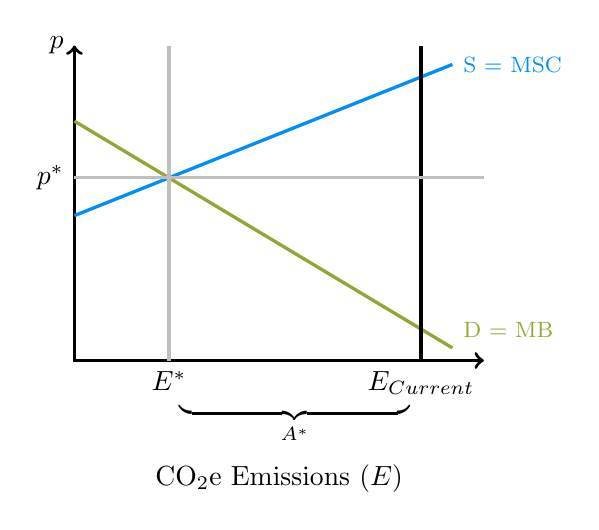
\begin{tikzpicture}[scale=0.4]
    \draw[very thick, <->] (0,10) node[left]{$p$} -- (0,0) -- (13,0);	
    \draw[very thick, color2, domain=0:12] plot(\x, {7.6 - .6*\x}) node[above right]{\footnotesize D = MB};
    \draw[very thick, color1, domain=0:12] plot(\x, {4.6 + .4*\x}) node[right]{\footnotesize S = MSC};
    \draw[very thick] (11, 0) node[below]{$E_\text{Current}$} -- (11, 10);
    \draw[very thick, lightgray] (3,0) node[below, black]{$E^*$} -- (3,10);
    \draw[very thick, lightgray] (0,5.8) node[left, black]{$p^*$} -- (13,5.8);	
    \node[below] at (6.5, -3) {CO$_2$e Emissions ($E$)};
    \draw (7, -2) node{$\underbrace{~~~~~~~~~~~~~~~~~~~~~~~~~}_{A^*}$};
\end{tikzpicture}
    
\end{frame}


\begin{frame}{Emissions Leakage}
  
\footnotesize
\centering
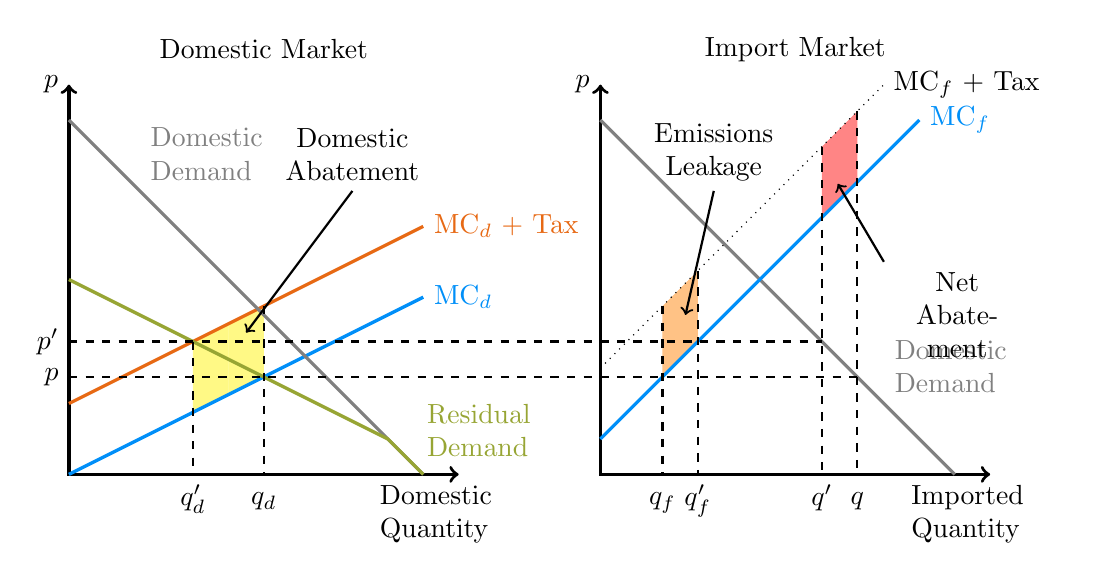
\begin{tikzpicture}[scale = 0.45]
    \draw[very thick, <->] (0, 11) node[left]{$p$} -- (0, 0) -- (11, 0) node[below, text width = 2cm]{Domestic Quantity};
    \draw[very thick, <->] (15, 11) node[left]{$p$} -- (15,0) -- (26, 0) node[below, text width = 2cm]{Imported Quantity};
    \fill[yellow!80!, opacity = 0.6] (3.5, 3.75) -- (3.5, 1.75) -- (4.5, 2.25) -- (4.5, 4.25) -- cycle;
    \fill[yellow!80!, opacity = 0.6] (4.5, 2.25) -- (5.5, 2.75) -- (5.5, 4.75) -- (4.5, 4.25) -- cycle;
    \fill[orange!80!, opacity = 0.6] (16.75, 4.75) -- (16.75, 2.75) -- (17.75, 3.75) -- (17.75, 5.75) -- cycle;
    %\fill[orange!80!, opacity = 0.6] (16.25, 4.25) -- (16.25, 2.25) -- (16.75, 2.75) -- (16.75, 4.75) -- cycle;
    \fill[red!80!, opacity = 0.6] (21.25, 9.25) -- (21.25, 7.25) -- (22.25, 8.25) -- (22.25, 10.25) -- cycle;
    %\fill[red!80!, opacity = 0.6] (20.75, 8.75) -- (20.75, 6.75) -- (21.25, 7.25) -- (21.25, 9.25) -- cycle;
    \draw[very thick, color1] (0,0) -- (10, 5) node[right]{MC$_d$};
    \draw[very thick, color3] (0,2) -- (10, 7) node[right]{MC$_d$ $+$ Tax};
    \draw[very thick, gray] (0, 10) -- (10,0) node[pos=.2, above right,text width = 1.5cm]{Domestic Demand}; 
    \draw[very thick, color2] (0,5.5) -- (9, 1) -- (10, 0) node[pos=.8, above right, text width = 1.5cm]{Residual Demand};
    %\draw[very thick, color2] (0, 6.5) -- (7,3) -- (10, 0);
    \draw[very thick, gray] (15, 10) -- (25, 0) node[pos=.8, above right,text width = 1.5cm]{Domestic Demand}; 
    \draw[very thick, color1] (15, 1) -- (24, 10) node[right, text width = 1.5cm]{MC$_f$};
    \draw[dashed, thick] (5.5, 4.75) -- (5.5, 0) node[below, yshift = -3pt]{$q_d$};
    \draw[dashed, thick] (3.5, 3.75) -- (3.5, 0) node[below]{$q_d'$};
    %\draw[dashed, thick] (4.5, 4.25) -- (4.5, 0) node[below]{$q_d''$};
    \draw[dashed, thick] (0, 3.75) node[left]{$p'$} -- (21.25, 3.75);
    \draw[dashed, thick] (0, 2.75) node[left]{$p$} -- (22.25, 2.75);
    %\draw[dashed, thick] (0,4.25) node[left]{$p''$} -- (20.75, 4.25);
    \draw[dashed, thick] (16.75,4.75) -- (16.75, 0) node[below, yshift = -3pt]{$q_f$};
    \draw[dashed, thick] (17.75, 5.75) -- (17.75, 0) node[below]{$q_f'$};
    %\draw[dashed, thick] (16.25, 4.25) -- (16.25, 0) node[below]{$q_f''$};
    \draw[dashed, thick] (22.25, 10.25) -- (22.25, 0) node[below, yshift = -3pt]{$q$};
    \draw[dashed, thick] (21.25, 9.25) -- (21.25, 0) node[below]{$q'$};
    %\draw[dashed, thick] (20.75, 8.75) -- (20.75, 0) node[below]{$q''$};
    \draw[dotted] (15, 3) -- (23, 11) node[right]{MC$_f$ $+$ Tax};
    \draw[thick, <-] (5, 4) -- (8, 8) node[above, text width = 2cm, align=center]{Domestic Abatement};
    \draw[thick, <-] (17.4, 4.5) -- (18.2, 8) node[above, text width = 2cm, align=center]{Emissions Leakage}; 
        \draw[thick, <-] (21.7, 8.2) -- (23, 6) node[below right, text width = 1.6cm, align=center]{Net Abatement};
        \node at (5.5, 12) {Domestic Market};
        \node at (20.5, 12) {Import Market}; 
\end{tikzpicture}

\end{frame}


\begin{frame}{Gobal Air Pollution v. Local Air Pollution}
    
    \begin{columns}
    \begin{column}{0.5\textwidth}
        \textbf{Global Air Pollutants}
        \vspace*{1em}
        \begin{itemize}
            \item Carbon dioxide (CO$_2$), Methane (CH$_4$), Nitrous oxide (N$_2$O)
            \vspace*{2em}
            \item Primarily long-run consequences
            \vspace*{2em}
            \item Location does not matter
        \end{itemize}
    \end{column}
    \begin{column}{0.5\textwidth}
        \textbf{Local Air Pollutants}
        \vspace*{1em}
        \begin{itemize}
            \item Nitrogen oxides (NO$_x$), Sulfur dioxide (SO$_2$), Particulate matter (PM2.5)
            \vspace*{1em}
            \item Mix of long- and short-run consequences
            \vspace*{1em}
            \item Location does matter
        \end{itemize}
    \end{column}
    \end{columns}
    
\end{frame}
    

\begin{frame}{Motivation \& Ex-Post Research}
    
    \begin{itemize}
        \item \href{https://ww2.arb.ca.gov/resources/documents/faq-cap-and-trade-program}{CARB Cap-and-Trade FAQ Page} 
        \vfill 
        \item Descriptive Analysis: Yes, California's cap-and-trade program increased disparities \citep{cushing2018carbon, pastor2022up}
        \vfill
        \item Causal Analysis: No, California's cap-and-trade program decreased disparities \citep{hernandez2023environmental}
    \end{itemize}

\end{frame}


\begin{frame}{Methodological Contributions}
    
\begin{itemize}
    \item Ex-ante model to anticipate changes in air pollution disparities
    \vfill 
    \item \emph{How} do carbon pricing policies shift local air pollution across jurisdictions?
    \vfill
    \item \cite{weber2021dynamic} creates a similar model, but does not:
    \begin{enumerate}
        \item Formally model disparities in air pollution concentrations
        \item Consider leakage and the redistribution outside of California
    \end{enumerate}
\end{itemize}

\end{frame}

% \begin{frame}{}
    
% \begin{itemize}
%     \item \emph{How} do carbon pricing policies lead to changes in air pollution concentration disparities?
%     \vfill 
%     \item \emph{How} do carbon pricing policies shift local air pollution across jurisdictions?
%     \vfill 
%     \item Contributions:
%     \begin{itemize}
%         \item Predictive framework for the effect of carbon pricing within the electric power industry on local air pollution disparities 
%         \item Demonstrate the importance of considering disparities across jurisdictions
%     \end{itemize}
% \end{itemize}

% \end{frame}


\sectiontocslide{Modeling Carbon Pricing \& Environmental Inequality}


\begin{frame}{Model Overview}

\begin{description}
    \item[Agents] $N$ fossil fuel power plants
    \vfill
    \item[Environ.]\begin{itemize}
        \item Geography: $R$ regions, each with its own wholesale market for electricity
        \item Constraints: Demand, (Capacity,) Transmission
        \item Markets: Perfectly competitive
    \end{itemize}  
    \vfill 
    \item[Actions]\begin{enumerate}
        \item Initial investment decision
        \item Hourly generation decisions
    \end{enumerate}
    \vfill
    \item[Behavior] Maximize discounted sum of future profits
    \vfill
    \item[Equilibrium] Minimize total investment and generation costs $\to$ Generation outcomes $\to$ Air pollution disparity outcomes 
\end{description}

\end{frame}


\begin{frame}{Action 1: Investment Decision}

\emph{Heat Rate}: How efficiently can a generator turn combustion into electricity?
\begin{itemize}
    \item $\rho_i$ : Power plant $i$'s heat rate (Btu/kWh)
    \item Affects both costs and emissions
\end{itemize}

\vfill
Action 1: Power plant $i$ chooses a level of investment $j_i$ to decrease its heat rate
\begin{itemize}
    \item Decrease generation costs in future periods
    \item Incurs a current cost for investment of $\Gamma(j_i)$
\end{itemize}

\end{frame}


\begin{frame}{Action 2: Operating Decision(s)}
    
Action 2: Power plant $i$ chooses whether or not to operate in period $t$, and if so, what regional wholesale market to sell its electricity on
\vfill 

\begin{equation}
    q_{itr} = \overline{q}_i \cdot \mathds{1}(r = a_{it})
\end{equation}
\vfill

Endogenous:
\begin{itemize}
    \item $a_{it}$ : Power plant $i$'s operating decision in time $t$, $a_{it} \in \{0, 1, \ldots, R\}$
\end{itemize}
Exogenous:
\begin{itemize}
    \item $\overline{q}_i$ : Power plant $i$'s nameplate capacity (maximum generation) (kW)
\end{itemize}

\end{frame}




\begin{frame}{Marginal Costs}
    
\begin{equation}
    mc_{ir} = \rho_i(u_{f_i} + e_{f_i} \tau_r) = \underbrace{\rho_i u_{f_i}}_{\text{Fuel Cost}} + \underbrace{\rho_i e_{f_i} \tau_r}_{\text{Emissions Cost}}
\end{equation}

\vfill
Endogenous:
\begin{itemize}
    \item $\rho_i$ : Power plant $i$'s heat rate (Btu/kWh)
\end{itemize}
Exogenous:
\begin{itemize}
    \item $u_{f_i}$ : Power plant $i$'s unit fuel cost (\$/Btu)
    \item $e_{f_i}$ : Power plant $i$'s CO$_2$e emissions intensity (tonnes CO$_2$e/Btu)
    \item $\tau_r$ : Emissions price in region $r$ (\$/tonne CO$_2$e)
\end{itemize}

\end{frame}


\begin{frame}{Equilibrium Generation in Period $t$}
    
\begin{align}
    \begin{split} \label{C_star}
        C^*(j\mid \text{Demand}_t) = &\min_{a_t}  \left\{ C(a_t\mid j)\right\} \\
        &\text{s.t.} ~~\begin{cases}
            \quad \text{Market Clearing Constraints}\\
            \quad \text{Transmission Constraints}\\
        \end{cases}
    \end{split}
\end{align}

\vfill
Given the profile of investment decisions $j$, choose the profile of operating decisions that minimizes total costs $C(a_t \mid j)$ in period $t$

\end{frame}


\begin{frame}{Equilibrium Investment in Period $0$}
    
\begin{equation}
    j^* = \arg\min_{j \in \mathcal{J}^N} \biggl\{ 
    \underbrace{\Gamma (j)}_{\substack{\text{Investment}\\ \text{Phase Costs}}} + \underbrace{\sum_{t=0}^T \delta^t C^*(j\mid \text{Demand}_t^e)}_{\text{Generation Phase Costs}}  \biggr\}
\end{equation}

\vfill
Choose the profile of investment decisions $j$ that minimizes the sum of investment costs and discounted equilibrium generation costs. 

\end{frame}


\begin{frame}{Generation Outcomes $\to$ Air Pollution Concentration Disparities}
    
For air pollutant $w$, power plant $i$'s period $t$ emissions are:
\begin{equation}
    w_{it}^* = e_i^w \rho_i^* q_{it}^*
\end{equation}

\vfill
Endogenous:
\begin{itemize}
    \item $\rho_i^*$ : Power plant $i$'s equilibrium heat rate (Btu/kWh)
    \item $q_{it}^*$ : Power plant $i$'s equilibrium generation in period $t$ (kWh)
\end{itemize}
Exogenous:
\begin{itemize}
    \item $e_i^w$ : Power plant $i$'s emissions intensity for pollutant $w$ (tonnes $w$/Btu)
\end{itemize}

\vfill
Create a nondescript function that maps power plant $i$'s generation in period $t$ to changes in the concentration of $w$ in all communities

\end{frame}


\begin{frame}{The Environmental Inequality Gap (EI Gap)}
    
Divide $M$ communities into two groups: Disadvantaged communities (DAC) and Non-Disadvantaged Communities (non-DAC)

\vfill
\begin{block}{The EI Gap}
    Let $\Phi_w^A(T)$ denote the average equilibrium concentration of air pollutant $w$ in a group of communities $A$ after $T$ periods. Then the EI Gap for pollutant $w$ after $T$ periods is defined by:
    \begin{equation}
        \text{EIGap}_w = \Phi_w^\text{DAC}(T) - \Phi_w^\text{non-DAC}(T).
    \end{equation}
\end{block}

\end{frame}


\begin{frame}{Model Takeaways}

Everything goes back to marginal costs:
\begin{equation*}
    mc_{ir} = \rho_i(u_{f_i} + e_{f_i} \tau_r)
\end{equation*}

\vfill
Apart from small changes due to investment, we only get redistribution of generation and emissions through relative changes along the supply curve (marginal costs)

\vfill
\begin{enumerate}
    \item $\Delta e_f$  :  $\uparrow \tau_r ~~\Rightarrow ~~ \uparrow \Delta e_f \tau_r ~~\Rightarrow ~~ \uparrow \Delta mc$
    \item $\Delta \tau_r$  :  $\uparrow \tau_r ~~\Rightarrow ~~ \uparrow \Delta \tau_r ~~\Rightarrow ~~ \uparrow \Delta mc$ \hfill (New!)
\end{enumerate}

\end{frame}



\sectiontocslide{Empirical Strategy \& Data}


\begin{frame}{Simulation Environment}
    
\begin{columns}
    \begin{column}{0.5\textwidth}
    
    \begin{itemize}
        \item Simulate generation across the Western US power grid (Western Interconnection)
        \vspace*{1em}
        \item Focus only on fossil fuel generation: coal, (natural) gas, oil
    \end{itemize}    

    \end{column}
    \begin{column}{0.5\textwidth}
        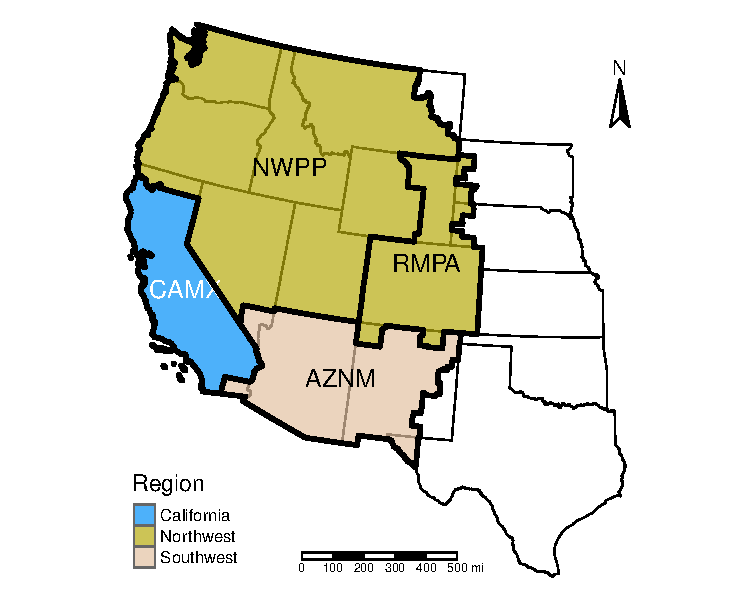
\includegraphics[width = \textwidth]{figures/chapter3_figures/WECC_map.pdf}
    \end{column}
\end{columns}

\end{frame}


\begin{frame}{Simulation Policy Scenarios}
    
    \begin{columns}
        \begin{column}{0.5\textwidth}
            \begin{itemize}
                \item Border Carbon Adjustments (BCAs): ``Carbon tariff'' on electricity California imports from elsewhere
                \vspace*{1em}
                \item Nine policy scenarios with a combination of BCAs and carbon prices
            \end{itemize}
        \end{column}
        \begin{column}{0.5\textwidth}
            \footnotesize
            \centering
            \begin{tabular}{c c c}
                \hline\hline
                Scenario & BCA? & Tax (\$/tonne)\\
                \hline
                A & No & 0\\
                B & No & 20\\
                C & No & 40\\
                D & No & 60\\
                E & No & 80\\
                F & Yes & 20 \\
                G & Yes & 40 \\
                H & Yes & 60 \\
                I & Yes & 80 \\
            \hline    
            \end{tabular}
        \end{column}
    \end{columns}

\end{frame}


\begin{frame}{$k$-Means Clustering}
    
\begin{itemize}
    \item Problem: Constrained optimization problems are too large
    \vfill
    \item Generation Problem
    \begin{itemize}
        \item Simplify $N$: $k$-means cluster power plants into thirty groups
    \end{itemize}
    \vfill 
    \item Investment Problem
    \begin{itemize}
        \item Simplify $T$: $k$-means cluster electricity demand into a ``representative day''
        \item Simplify $N$: $k$-means cluster generation clusters into four clusters
    \end{itemize}
\end{itemize}

\end{frame}


\begin{frame}{Generation $\to$ Pollutant Concentrations}

\begin{itemize}
    \item Most basic measure of concentration: tonnes of pollutant $w$ per square mile
    \vfill 
    \item EI Gap implementation:
    \begin{equation}\footnotesize
        \text{EIGap}_w = \text{Mean}_\text{DAC}\left[ \frac{\text{Annual Emissions}}{\text{Area}}\right] - \text{Mean}_\text{non-DAC}\left[ \frac{\text{Annual Emissions}}{\text{Area}}\right]
    \end{equation}
    \vfill

    \item Forthcoming: Census tracts + buffer zones
\end{itemize}

\end{frame}


\begin{frame}{Generation Data}
    
    Power Plants
    \begin{itemize}
        \item 2019 Emissions \& Generation Resource Integrated Database (eGRID) from the EPA
        \item All power plants with capacity $\geq 1$ MW
        \item Initial heat rates, emissions factors, locations, fuel types
    \end{itemize}

    \vfill
    Electricity Demand
    \begin{itemize}
        \item 2019--2021 EIA's Hourly Electric Grid Monitor Regional Files
        \item Regional demand at every hour and generation by fuel type
        \item Compute residual demand for each hour
    \end{itemize}

\end{frame}


\begin{frame}{Disadvantaged Communities}

Disadvantaged Communities in California:   
\begin{itemize}
    \item California SB 535 requires Census tracts to be designated as ``Disadvantaged'' or not to allocate revenue generated by the cap-and-trade program
    \item State develops a metric called CalEnviroScreen and set of criteria to make designations
\end{itemize}

\vfill
Disadvantaged Communities outside of California:
\begin{itemize}
    \item Must define for the analysis
    \item Use data from EPA's Environmental Justice Screening tool to create similar metric and designate Census tracts with the analogous criteria
\end{itemize}

\end{frame}



\sectiontocslide{Simulation Results}


\begin{frame}{Generation}

\centering
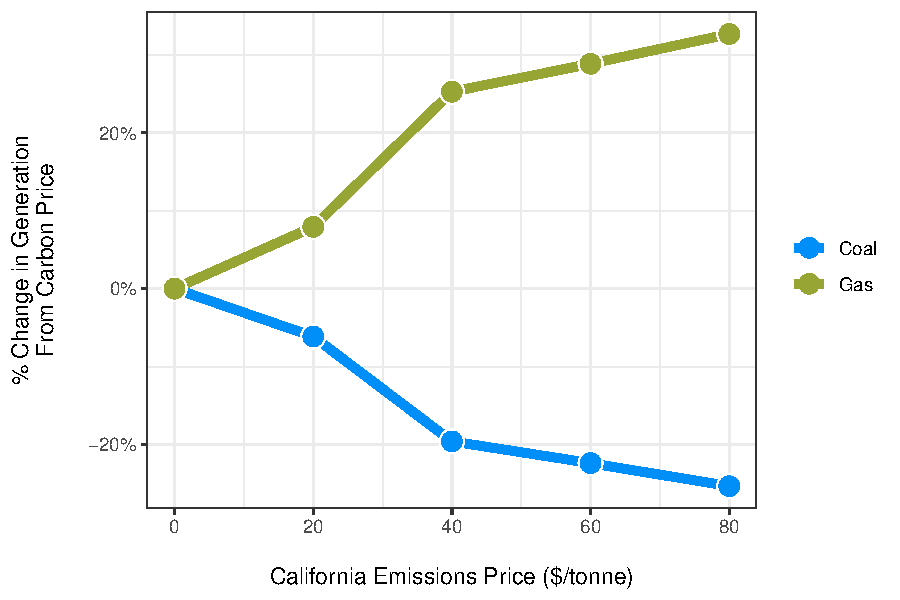
\includegraphics[width = 0.8\textwidth]{figures/chapter5_figures/gen_fuel_bca_pct.pdf}

\end{frame}


\begin{frame}{Greenhouse Gas Emissions}
    
\centering
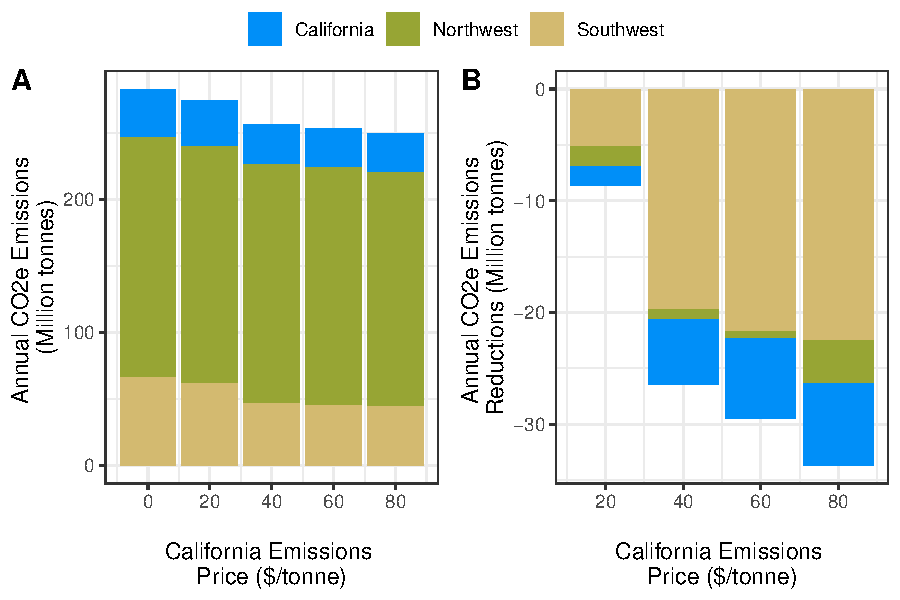
\includegraphics[width = 0.8\textwidth]{figures/chapter5_figures/sim_co2e_bca.pdf}

\end{frame}

\begin{frame}{Total NO$_x$ Emissions}

\centering
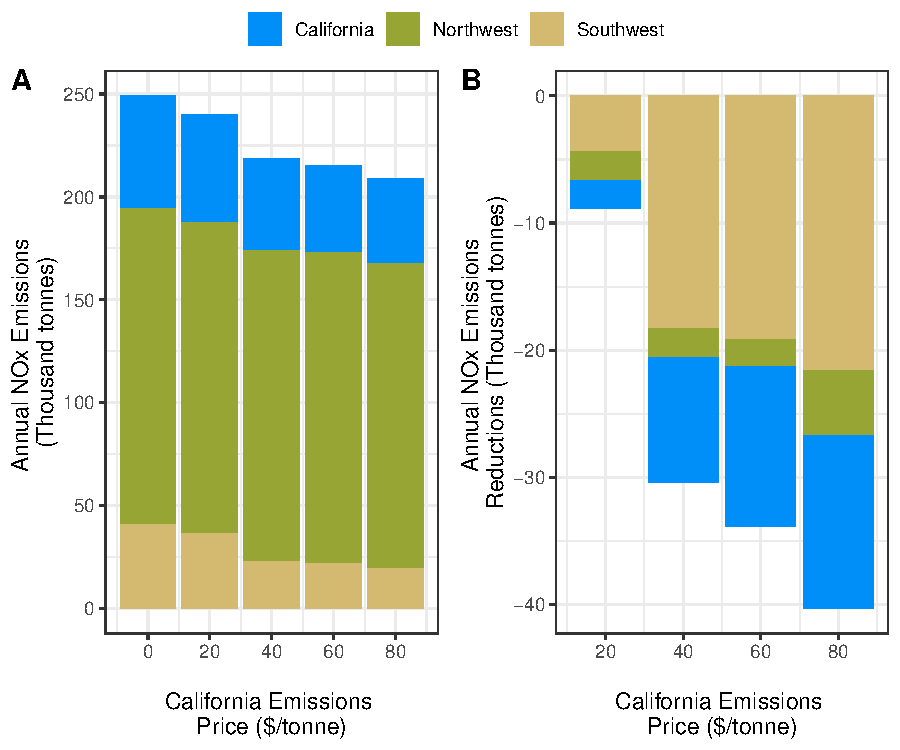
\includegraphics[width = 0.7\textwidth]{figures/chapter5_figures/sim_nox_bca.pdf}

\end{frame}

% \begin{frame}{Total PM2.5 Emissions}

% \centering
% 
\includegraphics[width = 0.7\textwidth]{figures/chapter5_figures/sim_pm25_bca.pdf}
        
% \end{frame}


\begin{frame}{The EI Gap (NO$_x$)}

\centering
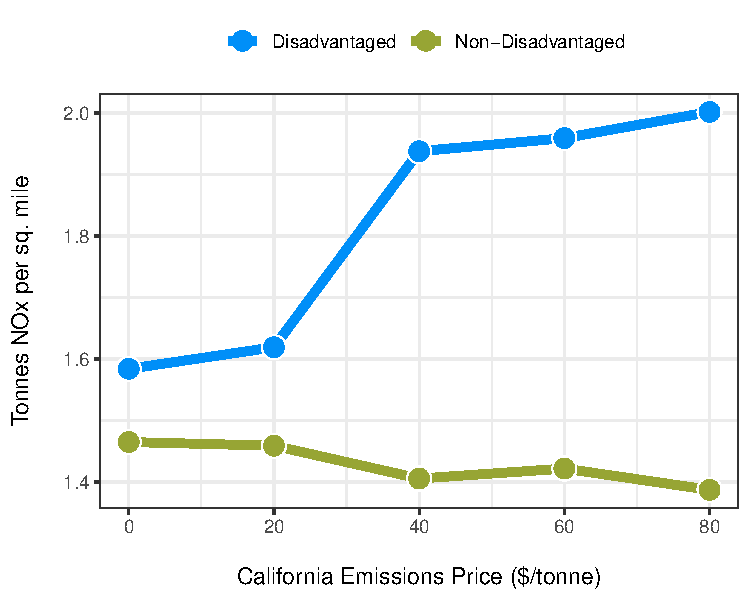
\includegraphics[width = 0.7\textwidth]{figures/chapter5_figures/ei_gap_bca_nox.pdf}

\end{frame}


\begin{frame}{The EI Gap (NO$_x$) in California}

\centering
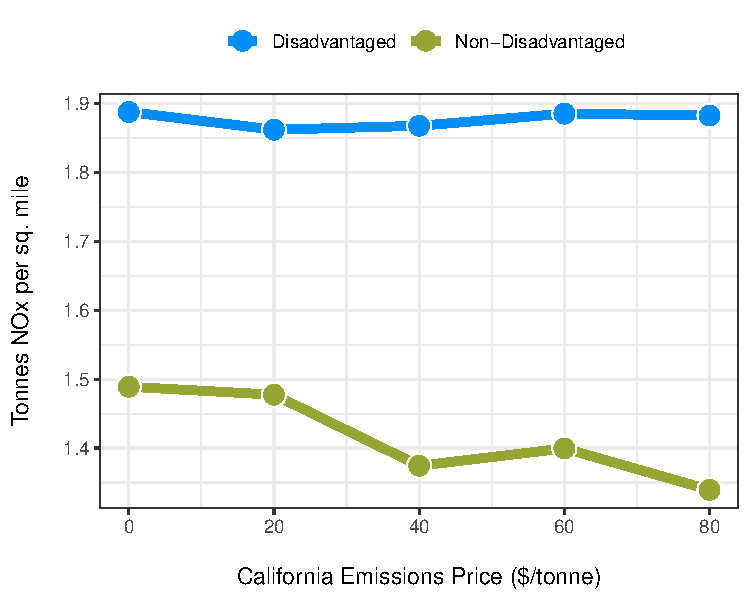
\includegraphics[width = 0.7\textwidth]{figures/chapter5_figures/ei_gap_bca_nox_cal.pdf}

\end{frame}


\begin{frame}{Unpacking the EI Gap (NO$_x$)}
    
Overall EI Gap (\$0 $\to$ \$80 per tonne):
\begin{itemize}
    \item NO$_x$ Concentration in DACs: $\uparrow 26.4\%$
    \item NO$_x$ Concentration in non-DACs: $\downarrow 5.3\%$
    \item EI Gap: $\uparrow 416\%$
\end{itemize}

\vfill
California EI Gap (\$0 $\to$ \$80 per tonne):
\begin{itemize}
    \item NO$_x$ Concentration in DACs: $\downarrow 0.3\%$
    \item NO$_x$ Concentration in non-DACs: $\downarrow 10.1\%$
    \item EI Gap: $\uparrow 36.2\%$
\end{itemize}


\end{frame}


\begin{frame}{EI Gap (Others)}

\centering
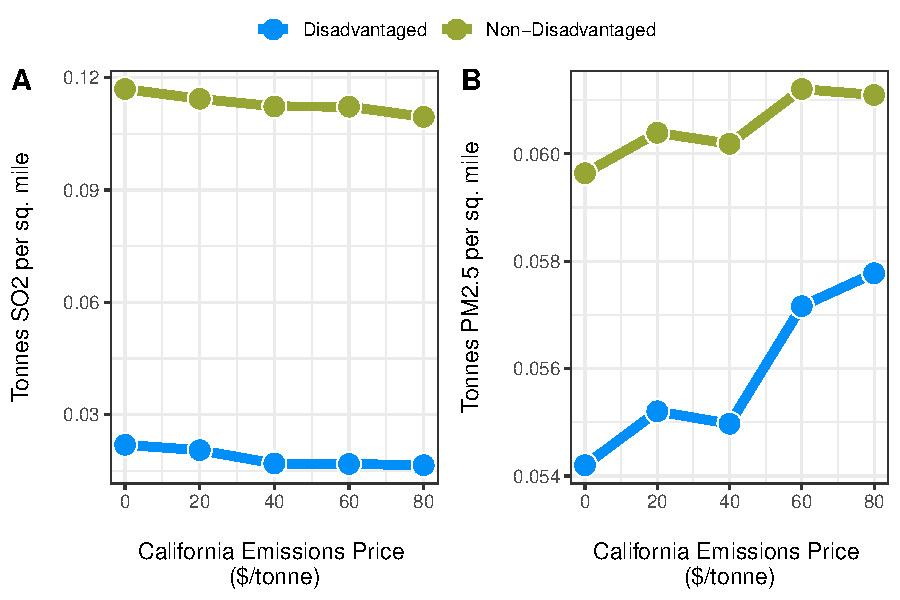
\includegraphics[width = 0.8\textwidth]{figures/chapter5_figures/ei_gap_so2_pm25.pdf}

\end{frame}


\sectiontocslide{Takeaways \& Discussion}


\begin{frame}{Simulation Upshots}

\begin{enumerate}
    \item Carbon pricing \emph{does} have the potential to exacerbate disparities in air pollution concentrations 
    \vfill
    \item Need more research that grapples with more intricate policy scenarios---namely combinations of cap-and-trade and localized pollution controls
    \vfill 
    \item Accounting for redistribution outside of the regulated jurisdiction matters
\end{enumerate}
    
\end{frame}


\begin{frame}{Limitations \& Future Work}

What is next for me:
\begin{itemize}
    \item Copyediting
    \item Diagnostics
    \item Alternative concentration measurements
    \item Expanding discussion of results
\end{itemize}

\vfill
What would be ideal:
\begin{itemize}
    \item Better modeling of air pollution concentrations
    \item Simulate more nuanced policies/more accurate counterfactuals
\end{itemize}

\end{frame}


\begin{frame}[allowframebreaks]{References}
\footnotesize

\bibliography{references}

\end{frame}


\begin{frame}{Greenhouse Gas Emissions Intensities}

\centering
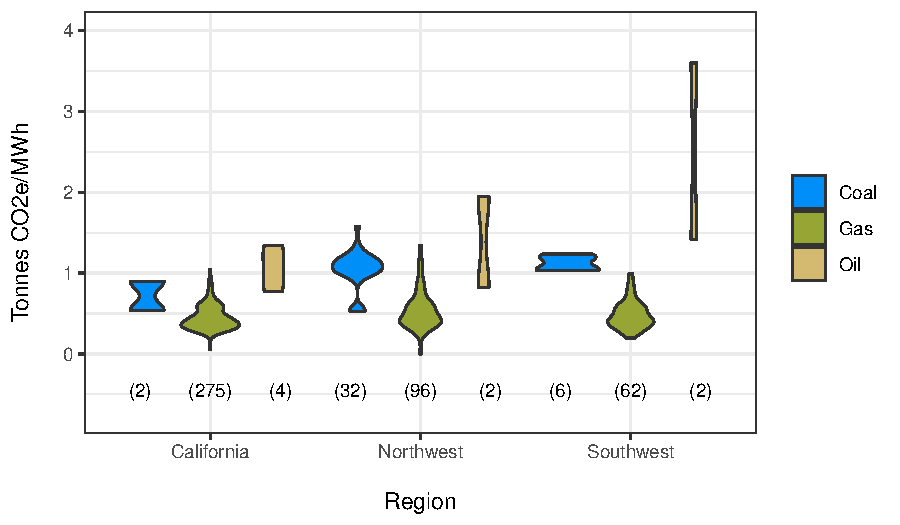
\includegraphics[width = 0.9\textwidth]{figures/chapter5_figures/EI_region_violin.pdf}
    
\end{frame}

\begin{frame}{Local Pollutant Emissions Intensities}

    \centering
    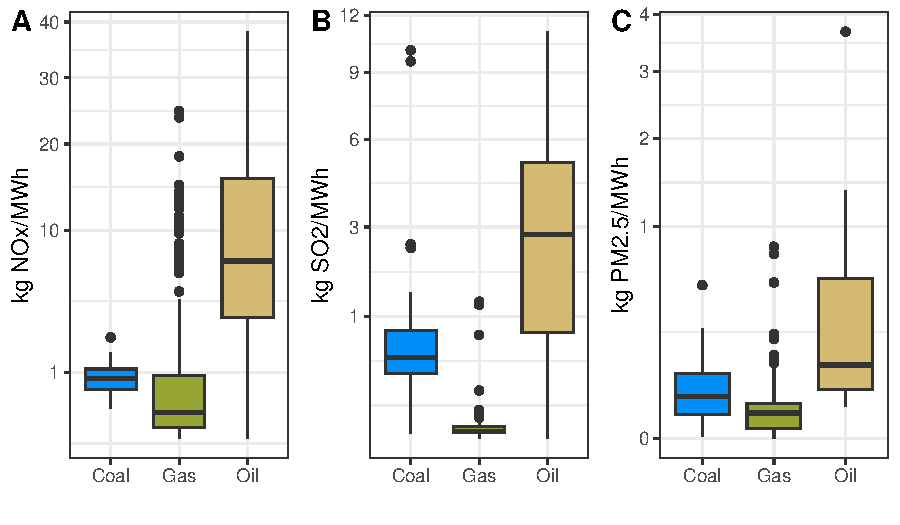
\includegraphics[width = 0.9\textwidth]{figures/chapter5_figures/local_poll_EI.pdf}
        
\end{frame}

\begin{frame}{Total SO$_2$ Emissions}

    \centering
    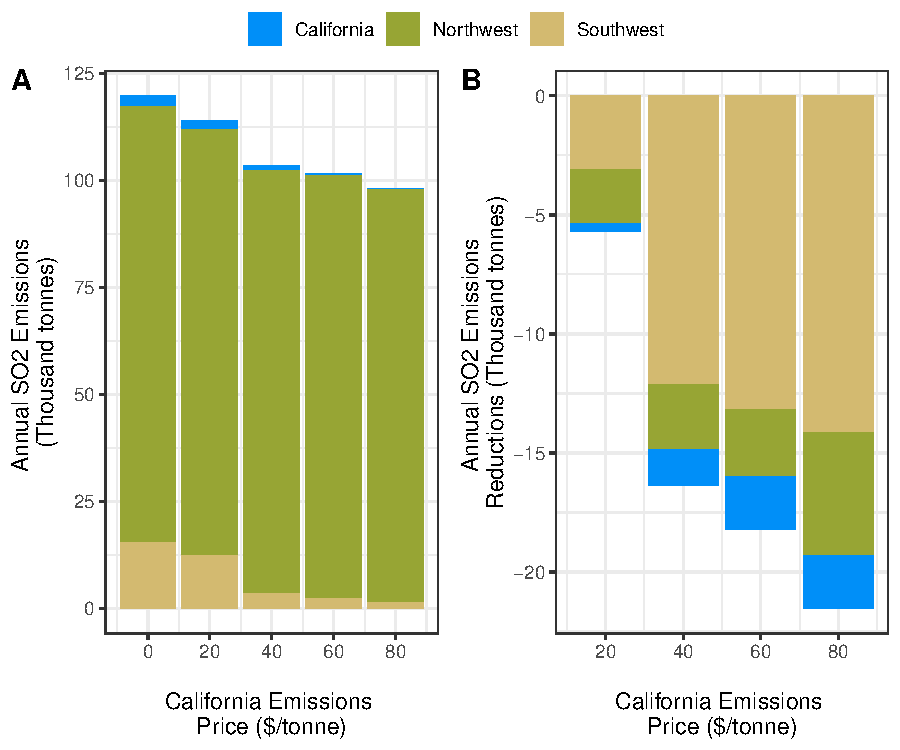
\includegraphics[width = 0.7\textwidth]{figures/chapter5_figures/sim_so2_bca.pdf}
        
\end{frame}



\end{document}